\documentclass[11pt]{article}
\usepackage{graphicx}
\usepackage{float}

\newcommand{\yourname}{}
\newcommand{\yourcollaborators}{}

\def\comments{0}

%format and packages

%\usepackage{algorithm, algorithmic}
\usepackage{algpseudocode}
\usepackage{amsmath, amssymb, amsthm}
\usepackage{enumerate}
\usepackage{enumitem}
\usepackage{framed}
\usepackage{verbatim}
\usepackage[margin=1.0in]{geometry}
\usepackage{microtype}
\usepackage{kpfonts}
\usepackage{palatino}
	\DeclareMathAlphabet{\mathtt}{OT1}{cmtt}{m}{n}
	\SetMathAlphabet{\mathtt}{bold}{OT1}{cmtt}{bx}{n}
	\DeclareMathAlphabet{\mathsf}{OT1}{cmss}{m}{n}
	\SetMathAlphabet{\mathsf}{bold}{OT1}{cmss}{bx}{n}
	\renewcommand*\ttdefault{cmtt}
	\renewcommand*\sfdefault{cmss}
	\renewcommand{\baselinestretch}{1.06}
\usepackage[usenames,dvipsnames]{xcolor}
\definecolor{DarkGreen}{rgb}{0.15,0.5,0.15}
\definecolor{DarkRed}{rgb}{0.6,0.2,0.2}
\definecolor{DarkBlue}{rgb}{0.2,0.2,0.6}
\definecolor{DarkPurple}{rgb}{0.4,0.2,0.4}
\usepackage[pdftex]{hyperref}
\hypersetup{
	linktocpage=true,
	colorlinks=true,				% false: boxed links; true: colored links
	linkcolor=DarkBlue,		% color of internal links
	citecolor=DarkBlue,	% color of links to bibliography
	urlcolor=DarkBlue,		% color of external links
}

\usepackage[boxruled,vlined,nofillcomment]{algorithm2e}
	\SetKwProg{Fn}{Function}{\string:}{}
	\SetKwFor{While}{While}{}{}
	\SetKwFor{For}{For}{}{}
	\SetKwIF{If}{ElseIf}{Else}{If}{:}{ElseIf}{Else}{:}
	\SetKw{Return}{Return}
	

%enclosure macros
\newcommand{\paren}[1]{\ensuremath{\left( {#1} \right)}}
\newcommand{\bracket}[1]{\ensuremath{\left\{ {#1} \right\}}}
\renewcommand{\sb}[1]{\ensuremath{\left[ {#1} \right\]}}
\newcommand{\ab}[1]{\ensuremath{\left\langle {#1} \right\rangle}}

%probability macros
\newcommand{\ex}[2]{{\ifx&#1& \mathbb{E} \else \underset{#1}{\mathbb{E}} \fi \left[#2\right]}}
\newcommand{\pr}[2]{{\ifx&#1& \mathbb{P} \else \underset{#1}{\mathbb{P}} \fi \left[#2\right]}}
\newcommand{\var}[2]{{\ifx&#1& \mathrm{Var} \else \underset{#1}{\mathrm{Var}} \fi \left[#2\right]}}

%useful CS macros
\newcommand{\poly}{\mathrm{poly}}
\newcommand{\polylog}{\mathrm{polylog}}
\newcommand{\zo}{\{0,1\}}
\newcommand{\pmo}{\{\pm1\}}
\newcommand{\getsr}{\gets_{\mbox{\tiny R}}}
\newcommand{\card}[1]{\left| #1 \right|}
\newcommand{\set}[1]{\left\{#1\right\}}
\newcommand{\negl}{\mathrm{negl}}
\newcommand{\eps}{\varepsilon}
\DeclareMathOperator*{\argmin}{arg\,min}
\DeclareMathOperator*{\argmax}{arg\,max}
\newcommand{\eqand}{\qquad \textrm{and} \qquad}
\newcommand{\ind}[1]{\mathbb{I}\{#1\}}
\newcommand{\sslash}{\ensuremath{\mathbin{/\mkern-3mu/}}}

%mathbb
\newcommand{\N}{\mathbb{N}}
\newcommand{\R}{\mathbb{R}}
\newcommand{\Z}{\mathbb{Z}}
%mathcal
\newcommand{\cA}{\mathcal{A}}
\newcommand{\cB}{\mathcal{B}}
\newcommand{\cC}{\mathcal{C}}
\newcommand{\cD}{\mathcal{D}}
\newcommand{\cE}{\mathcal{E}}
\newcommand{\cF}{\mathcal{F}}
\newcommand{\cL}{\mathcal{L}}
\newcommand{\cM}{\mathcal{M}}
\newcommand{\cO}{\mathcal{O}}
\newcommand{\cP}{\mathcal{P}}
\newcommand{\cQ}{\mathcal{Q}}
\newcommand{\cR}{\mathcal{R}}
\newcommand{\cS}{\mathcal{S}}
\newcommand{\cU}{\mathcal{U}}
\newcommand{\cV}{\mathcal{V}}
\newcommand{\cW}{\mathcal{W}}
\newcommand{\cX}{\mathcal{X}}
\newcommand{\cY}{\mathcal{Y}}
\newcommand{\cZ}{\mathcal{Z}}

%theorem macros
\newtheorem{thm}{Theorem}
\newtheorem{lem}[thm]{Lemma}
\newtheorem{fact}[thm]{Fact}
\newtheorem{clm}[thm]{Claim}
\newtheorem{rem}[thm]{Remark}
\newtheorem{coro}[thm]{Corollary}
\newtheorem{prop}[thm]{Proposition}
\newtheorem{conj}[thm]{Conjecture}

\theoremstyle{definition}
\newtheorem{defn}[thm]{Definition}


\newcommand{\instructor}{Virgil Pavlu}
\newcommand{\hwnum}{8}
%\newcommand{\hwdue}{Wednesday, May 20 at 11:59pm via \href{https://gradescope.com/courses/229309}{Gradescope}}

\newtheorem{prob}{}
\newtheorem{sol}{Solution}

\definecolor{cit}{rgb}{0.05,0.2,0.45} 
\newcommand{\solution}{\medskip\noindent{\color{DarkBlue}\textbf{Solution:}}}

\begin{document}
{\Large 
\begin{center}{CS5800: Algorithms} --- \instructor \end{center}}
{\large
\vspace{10pt}
\noindent Homework~\hwnum \vspace{2pt}%\\
%Submit via \href{https://www.gradescope.com/courses/232127}{Gradescope}}
}

\bigskip
{\large \noindent Name: \yourname }

{\large \noindent Collaborators: \yourcollaborators}

\vspace{15pt}

{\large \noindent Instructions:}

\begin{itemize}

\item Make sure to put your name on the first page.  If you are using the \LaTeX~template we provided, then you can make sure it appears by filling in the \texttt{yourname} command.

\item Please review the grading policy outlined in the course information page.

\item You must also write down with whom you worked on the assignment.  If this changes from problem to problem, then you should write down this information separately with each problem.

\item Problem numbers (like Exercise 3.1-1) are corresponding to CLRS $3^{rd}$ edition.  While the  $2^{nd}$ edition  has  similar  problems  with  similar  numbers,  the  actual  exercises  and their solutions are different, so make sure you are using the $3^{rd}$ edition.

\end{itemize}

\newpage



\begin{prob} \textbf{(50 points)}
\end{prob}

\noindent Implement a hash for text.  Given a string as input,  construct a hash with words as keys, and word counts as values.  Your implementation should include:

\begin{itemize}
\item a hash function that has good properties for text

\item storage and collision management using linked lists

\item operations:  insert(key,value), delete(key), increase(key), find(key), list-all-keys
\end{itemize}

\noindent Output the list of words together with their counts on an output file.  For this problem,you  cannot  use  built-in-language  data structures  that  can  index  by  strings  (like  hashtables).  Use a language that easily implements linked lists, like C/C++.

\noindent You can test your code on “Alice in Wonderland” by Lewis Carroll, at \href{http://www.ccs.neu.edu/home/vip/teach/Algorithms/7_hash_RBtree_simpleDS/hw_hash_RBtree/alice_in_wonderland.txt}{link}.

\noindent The test file used by TA will probably be shorter.

\noindent Try these three values for $m = MAXHASH : 30, 300, 1000$. For each of these m values,
produce a histogram over the lengths of collision lists. You can also calculate variance
of these lengths.

\noindent If your hash is close to uniform in collisions, you should get variance close to zero, and
almost all list-lengths around $\alpha = n/m$.

\noindent If your hash has long lists, we want to know how many and how long, for example
print the lengths of the longest 10$\%$ of the lists.


\noindent \textbf{(Extra Credit)} Find a way to record not only word counts, but also the positions in text.  For each word, besides the count value, build a linked list with positions in the given text.  Output this list together with the count.

\solution


\begin{prob} \textbf{(50 points)}
\end{prob}

\noindent Implement  a  red-black  tree,  including  binary-search-tree  operations \textit{sort, search, min, max, successor, predecessor} and  specific  red-black  procedures \textit{rotation, insert, delete.}  The \textit{delete} implementation is \textbf{Extra Credit} (but highly recommended).
\\

\noindent Your code should take the input array of numbers from a file and build a red-black tree with this input by sequence of “inserts”.  Then interactively ask the user for an operational command like “insert x” or “sort” or “search x” etc, on each of which your code rearranges the tree and if needed produces an output.  After each operation also print out the height of the tree.
\\

\noindent You  can  use  any  mechanism  to  implement  the  tree,  for  example  with  pointers  and struct objects in C++, or with arrays of indices that represent links between parent and children.  You cannot use any tree built-in structure in any language.


\solution

\begin{prob} \textbf{Implement Skiplists 50 points}
\end{prob}
\noindent Study the skiplist data structure and operations. They are used for sorting values, but in a datastructure more effficient than lists or arrays, and more 
guaranteed than binary search trees.  
Review Slides \href{https://www.ccs.neu.edu/home/vip/teach/Algorithms/7_hash_RBtree_simpleDS/hw_hash_RBtree/skiplists.pdf}{skiplists.pdf}  and \href{https://people.ok.ubc.ca/ylucet/DS/SkipList.html}{Visualizer}.
The demo will be a sequence of operations (asked by TA) such as for example insert 20, insert 40, insert 10, insert 20, insert 5, insert 80, delete 20, insert 100, insert 20, insert 30, delete 5, insert 50, lookup 80, etc

\solution

\begin{prob} \textbf{(50 points)}
\end{prob}
\noindent Implement binomial heaps as described in class and in the book. You
should use links (pointers) to implement the structure as shown in the figure~\ref{fig:binomial_heap}. Your
implementation should include the operations: Make-heap, Insert, Minimum, Extract-
Min, Union, Decrease-Key, Delete.
\begin{figure}[H]
    \centering
    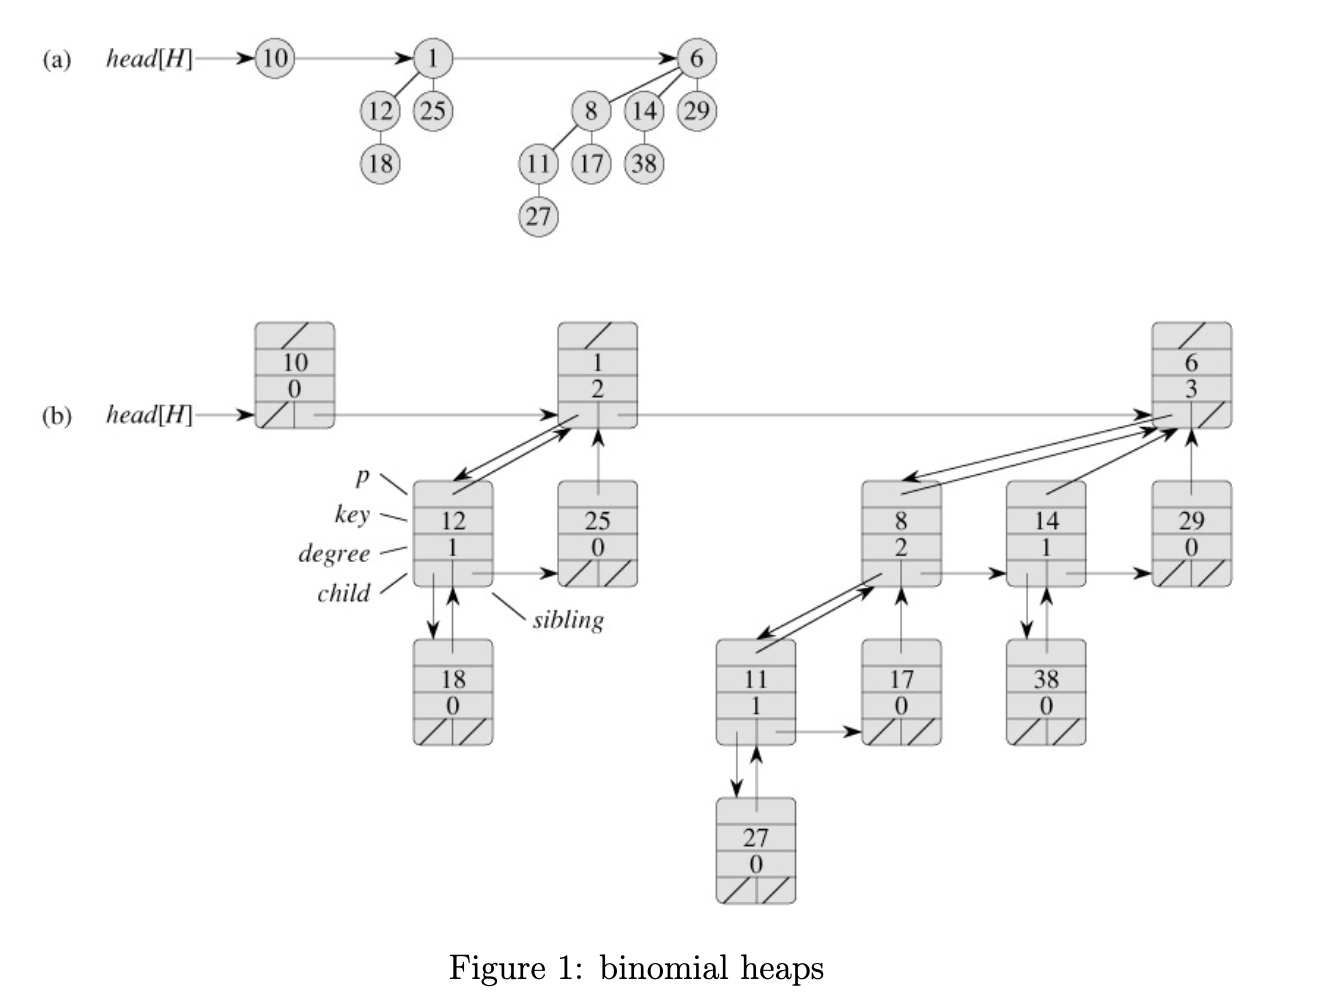
\includegraphics[width=1\linewidth]{image.png}
    
    \label{fig:enter-label}
\end{figure}
Make sure to preserve the characteristics of binomial heaps at all times: (1) each
component should be a binomial tree with children-keys bigger than the parent-key;
(2) the binomial trees should be in order of size from left to right. Test your code
with several arrays of randomly generated integers (keys).

\solution

\begin{prob} \textbf{16.3-3}
\end{prob}
\noindent Consider an ordinary binary min-heap data structure supporting the instructions \textsc{Insert} and \textsc{Extract-Min} that, when there are $n$ items in the heap, implements each operation in $O(\log n)$ worst-case time. Give a potential function $\Phi$ such that the amortized cost of \textsc{Insert} is $O(\log n)$ and the amortized cost of \textsc{Extract-Min} is $O(1)$, and show that your potential function yields these amortized time bounds. Note that in the analysis, $n$ is the number of items currently in the heap, and you do not know a bound on the maximum number of items that can ever be stored in the heap.

\solution

% Step 1: Define Variables and Basic Setup
\subsection*{1. Basic Definitions}
Let's understand what variables we're working with:
\begin{itemize}
  \item $D_i$ = the heap after $i$th operation
  \item $n_i$ = number of elements in $D_i$
  \item $k$ = constant for operation time bound
  \item Each INSERT or EXTRACT-MIN takes at most $k \ln n$ time
  \item where $n = \max(n_{i-1}, n_i)$
\end{itemize}
Note: We're using natural log because it will make our calculations cleaner (we'll see why later!)

% Step 2: Define Potential Function
\subsection*{2. The Potential Function}
First, let's define our potential function:
\[
\Phi(D_i) = \begin{cases}
0 & \text{if } n_i = 0, \\
kn_i \ln n_i & \text{if } n_i > 0.
\end{cases}
\]

Key properties:
\begin{itemize}
  \item Starts at zero: $\Phi(D_0) = 0$ (empty heap)
  \item Always non-negative: $\Phi(D_i) \geq 0$
\end{itemize}

% Step 3: Important Inequality Proof
\subsection*{3. Proving a Useful Inequality}
Before proceeding, we need to prove that for $n \geq 2$: $n \ln \frac{n}{n-1} \leq 2$

Let's break this down step by step:
\begin{align*}
n \ln \frac{n}{n-1} &= n \ln \left(1 + \frac{1}{n-1}\right) \\
&= \ln \left(1 + \frac{1}{n-1}\right)^n \\
&\leq \ln \left(e^{\frac{1}{n-1}}\right)^n & \text{(using } 1 + x \leq e^x\text{)} \\
&= \ln e^{\frac{n}{n-1}} \\
&= \frac{n}{n-1} \\
&\leq 2
\end{align*}

% Step 4: INSERT Operation Analysis
\subsection*{4. Analysis of INSERT Operation}

\subsubsection*{4.1 Inserting into Empty Heap}
When inserting into empty heap:
\begin{itemize}
  \item $n_i = 1$
  \item $n_{i-1} = 0$
\end{itemize}

Amortized cost calculation:
\begin{align*}
\hat{c_i} &= c_i + \Phi(D_i) - \Phi(D_{i-1}) \\
&\leq k \ln 1 + k \cdot 1 \ln 1 - 0 \\
&= 0
\end{align*}

\subsubsection*{4.2 Inserting into Nonempty Heap}
When inserting into nonempty heap ($n_i = n_{i-1} + 1 \geq 2$):
\begin{align*}
\hat{c_i} &= c_i + \Phi(D_i) - \Phi(D_{i-1}) \\
&\leq k \ln n_i + kn_i \ln n_i - kn_{i-1} \ln n_{i-1} \\
&= k \ln n_i + kn_i \ln n_i - k(n_i - 1)\ln(n_i - 1) \\
&= k \ln n_i + kn_i \ln n_i - kn_i \ln(n_i - 1) + k \ln(n_i - 1) \\
&< 2k \ln n_i + kn_i \ln \frac{n_i}{n_i - 1} \\
&\leq 2k \ln n_i + 2k & \text{(since } n_i \geq 2\text{)} \\
&= O(\lg n_i)
\end{align*}

% Step 5: EXTRACT-MIN Operation Analysis
\subsection*{5. Analysis of EXTRACT-MIN Operation}

\subsubsection*{5.1 Extracting Only Item}
When extracting the only item:
\begin{itemize}
  \item $n_i = 0$
  \item $n_{i-1} = 1$
\end{itemize}

Amortized cost:
\begin{align*}
\hat{c_i} &= c_i + \Phi(D_i) - \Phi(D_{i-1}) \\
&\leq k \ln 1 + 0 - k \cdot 1 \ln 1 \\
&= 0
\end{align*}

\subsubsection*{5.2 Extracting from Heap with Multiple Items}
When $n_i = n_{i-1} - 1$ and $n_{i-1} \geq 2$:
\begin{align*}
\hat{c_i} &= c_i + \Phi(D_i) - \Phi(D_{i-1}) \\
&\leq k \ln n_{i-1} + kn_i \ln n_i - kn_{i-1} \ln n_{i-1} \\
&= k \ln n_{i-1} + k(n_{i-1} - 1)\ln(n_{i-1} - 1) - kn_{i-1} \ln n_{i-1} \\
&= k \ln n_{i-1} + kn_{i-1} \ln(n_{i-1} - 1) - k\ln(n_{i-1} - 1) - kn_{i-1} \ln n_{i-1} \\
&= k \ln \frac{n_{i-1}}{n_{i-1} - 1} + kn_{i-1} \ln \frac{n_{i-1} - 1}{n_{i-1}} \\
&< k \ln \frac{n_{i-1}}{n_{i-1} - 1} + kn_{i-1} \ln 1 \\
&= k \ln \frac{n_{i-1}}{n_{i-1} - 1} \\
&\leq k \ln 2 & \text{(since } n_{i-1} \geq 2\text{)} \\
&= O(1)
\end{align*}

% Step 6: Alternative Potential Function
\subsection*{6. An Alternative Potential Function}
Let's look at another way to define the potential function:

For each node $x$ in heap:
\begin{itemize}
  \item Let $d_i(x)$ = depth of node $x$ in $D_i$
  \item Define:
\end{itemize}

\[
\Phi(D_i) = \sum_{x \in D_i} k(d_i(x) + 1)
\]
\[
= k\left(n_i + \sum_{x \in D_i} d_i(x)\right)
\]

Properties of this new function:
\begin{itemize}
  \item Initially $\Phi(D_0) = 0$ (empty set sum)
  \item Always $\Phi(D_i) \geq 0$
  \item After INSERT: changes by $k(1 + \lfloor\lg n_i\rfloor)$
    \begin{itemize}
      \item Amortized cost: $O(\lg n_i) + O(\lg n_i) = O(\lg n)$
    \end{itemize}
  \item After EXTRACT-MIN: decreases by $k(1 + \lfloor\lg n_{i-1}\rfloor)$
    \begin{itemize}
      \item Amortized cost: $k \lg n_{i-1} - k(1 + \lfloor\lg n_{i-1}\rfloor) = O(1)$
    \end{itemize}
\end{itemize}
\end{document}
